\section{Prepogibanje stožnic}
\label{pogl:stoznice}

% kako konstruiramo tangente na stožnice in zakaj konstrukcije tako delujejo
% parabola, elipsa, hiperbola
% povezava z O6
% pa omeni tudi O7, kjer je skupna tangenta na dve paraboli
% a za krožnico se tudi da?

Iz didaktičnega vidika zelo zanimivo poglavje nam predstavlja konstrukcije tangent na stožnice s prepogibanjem papirja. Vsebina je tu predstavljena tako, da je bralec najprej povabljen, da vzame list papirja in ga prepogiba po navedenih korakih. Po opažanju, kaj se na papirju pri tem prikaže, preidemo na matematični del, kjer dokažemo, da so prepogibi res tangente na določeno stožnico.

% Za vsako stožnico:
% 1. konstrukcija (navodila za prepogibanje)
% 2. matematični dokaz, zakaj so to ravno tangente
% kdo je izumil ta navodila in kdaj?
% je še kakšna druga metoda?

% na koncu še O7 -- konstrukcija skupne parabole na dve stožnice -- a se da iz tega še kaj pametnega izcimit?

\subsection{Parabola}

% Hull je našel Row-a (prvič izdana 1893) kot najstarejši zapis te konstrukcije
\textit{\textbf{Naloga:} Vzemi pravokoten list papirja in svinčnik ter nekje sredi spodnje polovice lista s pisalom označi točko. Nato si izberi točko še na spodnji stranici lista in ga prepogni tako, da se obe izbrani točki prekrijeta. To ponovi čimvečkrat (gl.\ sliko~\ref{fig:koraki_parabola}). Kaj opaziš?}

\begin{figure}[h]
    \centering
    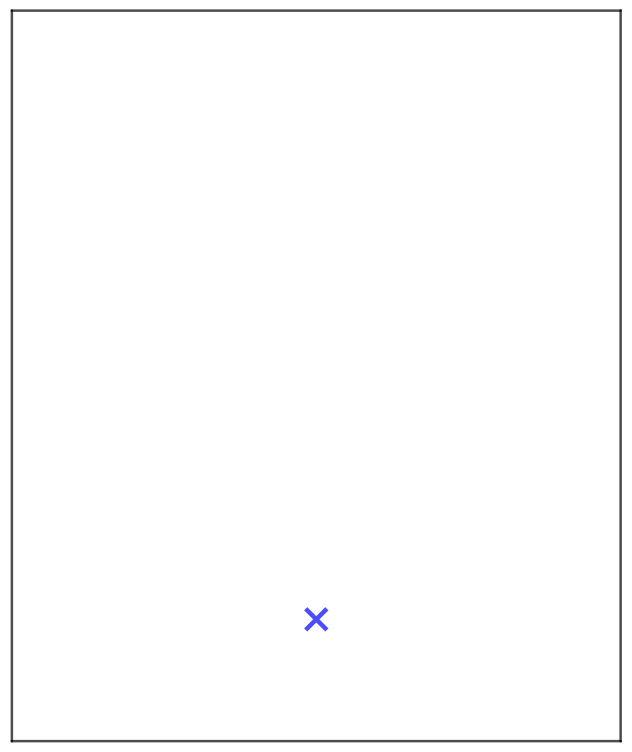
\includegraphics[width=0.3\textwidth]{images/stožnice/folding_parabola_1.png}
    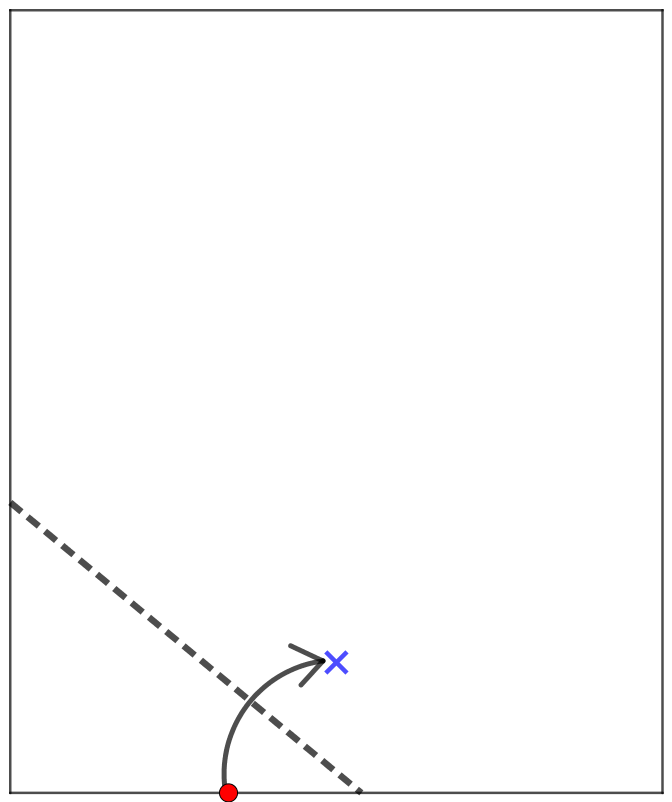
\includegraphics[width=0.3\textwidth]{images/stožnice/folding_parabola_2.png}
    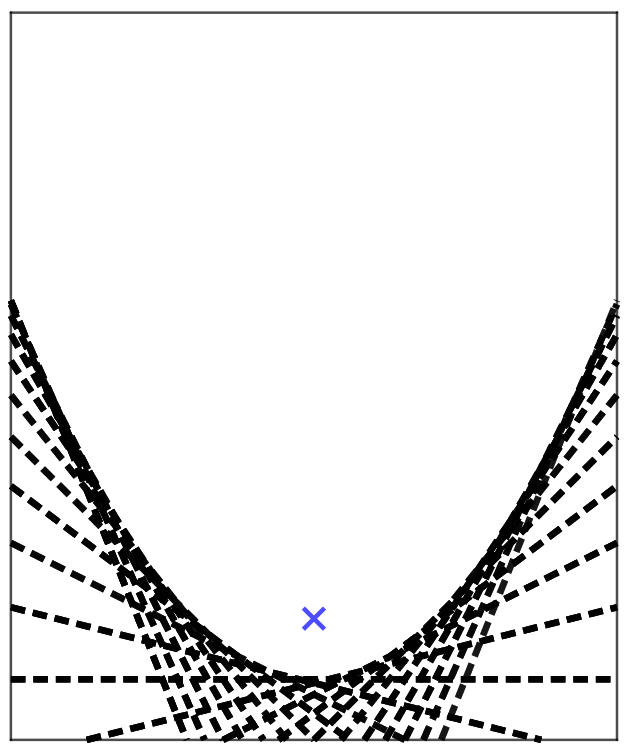
\includegraphics[width=0.3\textwidth]{images/stožnice/folding_parabola_3.png}
    \caption[Prepogibanje parabole]{Prepogibanje spodnje stranice papirja na izbrano točko.}
    \label{fig:koraki_parabola}
\end{figure}

Omenjen pregib je origami operacija~\ref{op:O3}, lahko pa nanjo gledamo tudi kot na operacijo~\ref{op:O6}. Za le-to smo v poglavju~\ref{pogl:aksiomi} že premislili, da nam pregib, ki poteka skozi dano točko $B$ in točko $A$ položi na premica $a$, poda tangento na parabolo z goriščem $A$ in premico vodnico $a$ (gl.\ sliko~\ref{fig:O6_parabola} in premislek nad njo). Tukaj pa take točke $B$ ni, kar pomeni le to, da smo s pregibom konstruirali neko tangento -- pregib je namreč simetrala daljice, ki ima za krajišči obe izbrani točki iz navodil naloge, torej obstaja točka (točka $P$ na sliki~\ref{fig:O6_parabola}), ki je enako oddaljena od spodnje stranice lista in prve izbrane točke. Nadaljni premislek, da je to edino presečišče pregiba in parabole, je enak kot prej.

Po večkrat izvedenih pregibih spodnje stranice lista na začetno izbrano točko dobimo na papirju obris krivulje. Ker so pregibi tangente na parabolo, predvidevamo, da je ta krivulja ravno parabola. Vendar moramo to dokazati. V ta namen si -- brez škode za splošnost, saj lahko z origamijem zrcalimo in rotiramo točke ter premice -- model poljubne točke in  spodnje stranice lista natančno določimo. Uporabimo že znan model iz dokaza izreka~\ref{izr:origami_konstruktibilnost} (pri konstrukciji $\sqrt{r}$): vzemimo točko $A(0, 1)$ in premico $a: y = -1$, ki sta origami-konstruktibilni, in naredimo pregib, ki točko $A$ preslika na premico $a$ v točko $A'(t, -1)$ za nek $t \in \R$ (slika~\ref{fig:enacba_tangente_par1}).

\begin{figure}[h]
    \centering
    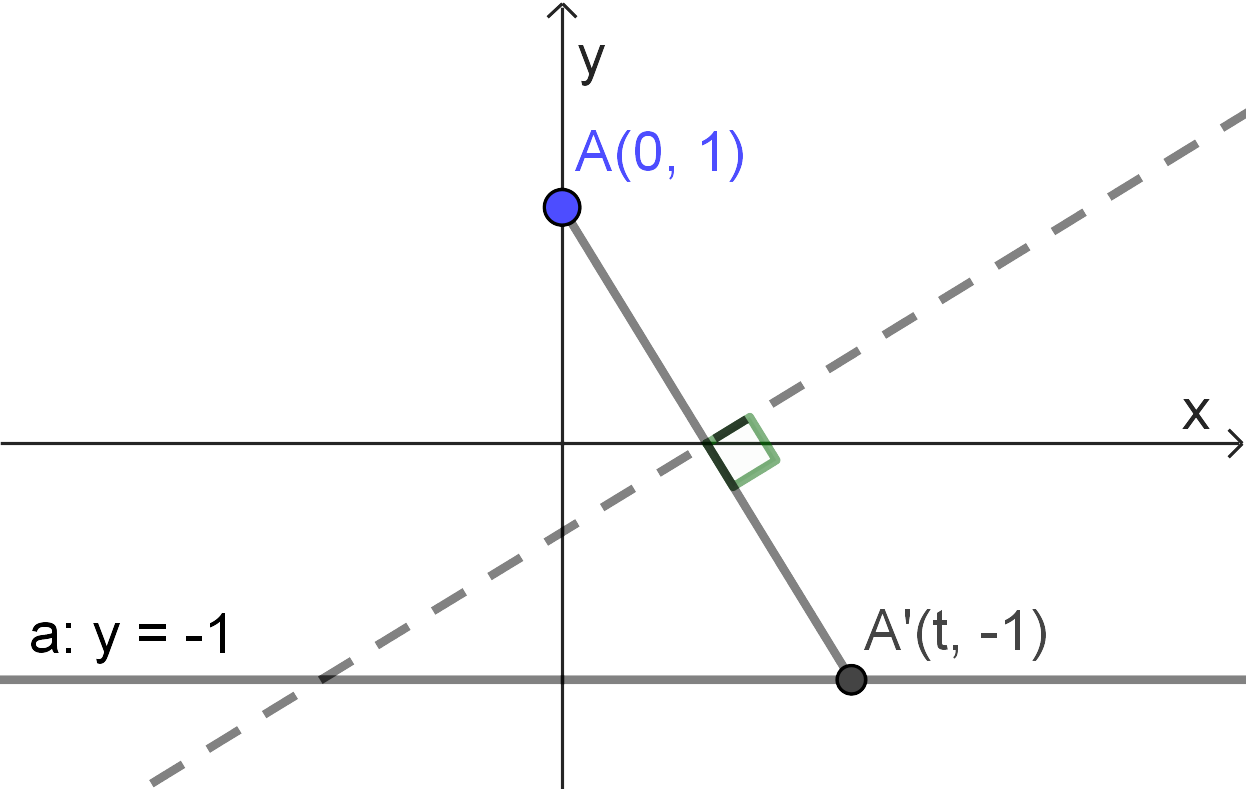
\includegraphics[width=0.5\textwidth]{images/enacba_parabole1.png}
    \caption[Enačba tangente na parabolo]{Pregib točke $A(0, 1)$ na premico $a: y = -1$.}
    \label{fig:enacba_tangente_par1}
\end{figure}

Ker je pregib oz.\ konstruirana premica simetrala daljice $AA'$, lahko hitro določimo njeno enačbo. Koeficient nosilke daljice $AA'$ je $k_A = -\frac{2}{t}$, središče pa $(\frac{t}{2}, 0)$. Tako hitro določimo enačbo pregiba:
\begin{equation}
    y = \frac{t}{2} x - \frac{t^2}{4}.
    \label{eq:tang_par}
\end{equation}
Dobili smo parametrizacijo neke družine premic. Za vsak $t \in \R$ torej dobimo drugo tangento na parabolo z goriščem v točki $A$ in premico vodnico $a$, ki ima zgornjo enačbo.

Za vse točke na pregibu velja, da so enako oddaljene od točk $A$ in $A'$. Vemo že, da pa je le ena točka $T$, da velja $d(T, A) = d(T, a)$. Zato je njena abscisa $x = t$ (točka $T$ leži na pregibu točno nad točko $A'$). Ko to vstavimo v enačbo~\ref{eq:tang_par}, dobimo še ordinato $y = t^2 / 4$. Ker točka $T$ za vsak $t \in \R$ leži na paraboli, pri menjavi $x = t$ dobimo njeno enačbo: $y = x^2 / 4$.

Vendar to ni dokaz, da je obris pregibov iz naloge res parabola. Zgornji premislek temelji na že znanem dejstvu, da so pregibi tangentni na parabole, vendar nam nič ne zagotavlja, da take točke $T$ ležijo točno na obrisu.

Hull v~\cite[str.\ 55--56]{hull2013} poda naslednji dokaz preko kvadratne formule. Iz poglavja~\ref{pogl:aksiomi} vemo, da pregib~\ref{op:O6} ne obstaja vedno (slika~\ref{fig:O6} desno). Poglejmo, ali obstajajo v ravnini našega modela kakšne točke, skozi katere ne moremo konstruirati pregiba oz.\ tangente. Vzemimo našo parametrizacijo družine tangent (enačba~\ref{eq:tang_par}). Če jo rešimo za $t$, nam dobljena formula pove, za katere vrednosti $t$ pregib poteka skozi točko $(x, y)$:
$$ \frac{1}{4}t^2 - \frac{x}{2}t + y = 0 \Rightarrow t_{1,2} = \frac{\frac{x}{2} \pm \sqrt{\frac{x^2}{4} - y}}{\frac{1}{2}}.$$
Enačba ima realne rešitve pri pogoju $\frac{x^2}{4} - y \geq 0$. Torej le točke iz območja, za katerega velja $y > x^2 / 4$, ne morejo ležati na nobenem izmed konstruiranih pregibov. Obris, ki ga dobimo v nalogi, je meja tega območja, torej ravno parabola $y = x^2 / 4$.

Torej je naš razmislek dva odstavka višje utemeljen. Sedaj, ko vemo, da je obris, ki nastane po večkratnem prepogibu spodnje stranice lista papirja na izbrano točko, res parabola, lahko pogledamo še več načinov za določitev enačbe parabole~\cite[str.\ 55--56]{hull2013}:
\begin{itemize}
    \item Naj bo $y(x)$ naša parabola, katere enačbo iščemo. Vemo, da je v našem modelu za poljuben $t \in \R$ pregib v neki točki $(x, y(x))$ tangenten na parabolo, koeficient tangente pa je $t / 2$. Očitno velja $x = t$, torej je koeficient kar $x / 2$. Zato dobimo
    $$ \frac{dy}{dx} = \frac{x}{2} \Rightarrow y = \frac{x^2}{4} + C. $$
    Ker parabola očitno vsebuje točko $(0, 0)$, je $C = 0$ in dobimo želeno enačbo $y = x^2 / 4$.
    \item 
\end{itemize}